\subsubsection{Overview}

This component is the interface for the Refbox. It handles the communication between the Refbox and the robotinos. Its functionality is very important, since communication to the Referee box is essential to receive game instructions and report sensed information to gain points. For a full understanding of the communication patterns, it is recommended to read the referee box manual located at \url{ http://www.robocup-logistics.org/refbox}. For message serialization over the IP channel between the Robotino and the Refbox, Google Protocol-Buffers are used. More information about this can be found at (\url{https://developers.google.com/protocol-buffers}). In the current state, the component implements most of the messages which are used at the Robocup competition.

\subsubsection{Situation in 2016}

In the 2016 version of the component, the RefBox Server component was not used to send back information about detected MPS \cite{BOK}. This means that a full communication path between the InstructionPlaner and Refbox was not implemented. Also a global Refbox software was not installed in the lab. 


\subsubsection{Situation in 2017}

In 2017, new objects like more zones and a new MPS station need to be handled by the Refbox Server. Therefore, new communication objects have been added. Receiving the team color, game phase and order contracts is working and tested. The connection from the Refbox to the Instruction Planner also works and was proven stable during the testing phase. The detection of the maintenance phase is now possible. Sending MPS information like the zone, orientation or type from the Refbox server to Referee Box computer works as it should. The Refbox adds successfully points for correct MPS reports and removes points for incorrect MPS reports. \\

To run the Refbox, it is necessary to modify the following parameters: the \textbf{HostIP} which is the IP address of the Referee Box, the \textbf{Name} which represents the name of the Robotino (this name will be listed on the Referee Box GUI), the \textbf{Number} which is the (jersey) number of the Robotino (this number will be listed at the referee box GUI) and the \textbf{Cryptokey} which is the key used for the encrypted team channel.\\

\subsubsection{Classes}

This section describes important C++ classes which are used in the Refbox Server. Reading the source code at the same time is recommended.\\

\begin{figure}[!h]
\centering
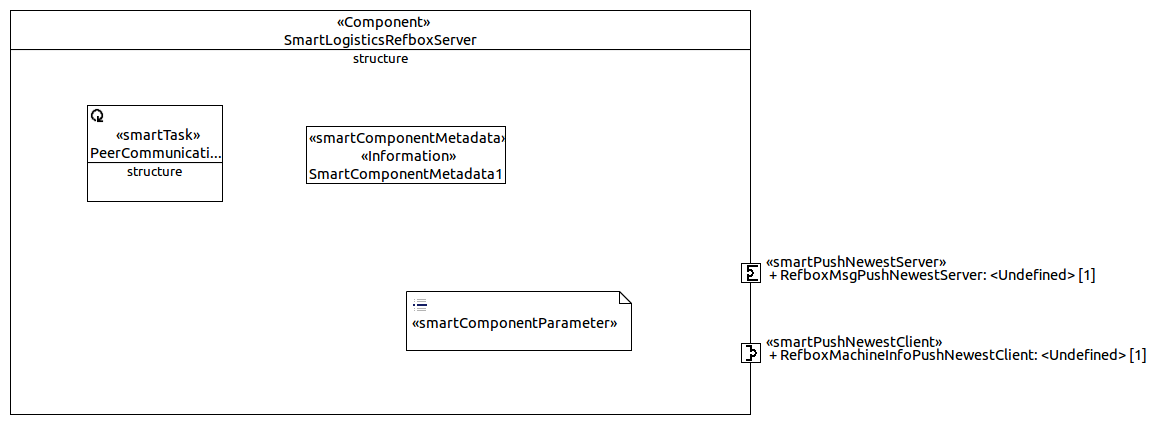
\includegraphics[width=\linewidth]{pic/component_refbox_server.png}
\caption{Model of Refbox server}
\label{fig:modelRefboxServer}
\end{figure}

First, the \textbf{RefboxPeer} class owns the instances of protobuf peers. One peer is created for the team channel and another one for the public channel. The peers are used to receive and send protobuf messages via the corresponding channels. Note that the robots never send information over the public channel, but only listen to it. All used protobuf messages must be registered in the peers message register. To handle all received messages, the peers are connected to a signal handler, which is represented by the class \textbf{CommunicationHandler}. \\

Next, the \textbf{CommunicationHandler} class permits to trigger the handle message method when a message is received from a connected peer. Depending on the type of the message, a specific evaluation method of the \textbf{MessageEvaluator} class is called to decode the message.\\

Then, the \textbf{MessageEvaluator} class has an overloaded method named \textbf{evaluate} which applies for any kind of message type. However, not all of the overloaded variants have been implemented so far. Until now, only the relevant message types needed for the exploration phase are completely realized (GameState and ExplorationInfo). Each variant is supposed to read the protobuf message and extract the most important information into the internal communication objects of type CommRefbox. Those are used to pass the relevant information to the instruction planner component. In the production phase, the evaluate method for the orderInfo message needs to be developed.\\

Next the \textbf{ConnectionMaintenance} class has a task which sends a beacon signal every two seconds via the team peer. This is the periodic heartbeat signal to the referee box, which makes the referee box aware of the presence of the robots. Therefore, also some information about the robot is contained in the message, such as its name, team name and number.\\

Finally, the \textbf{PeerCommunication} class is the components SmartTask of the SmartSoft environment. This means this is the loop construct which will be run as long as the component is active. At the current state, it does nothing more than sending new registered information about the gamestate or explorationinfo messages to the instruction planner via the push server.\\

\begin{figure}[!h]
\centering
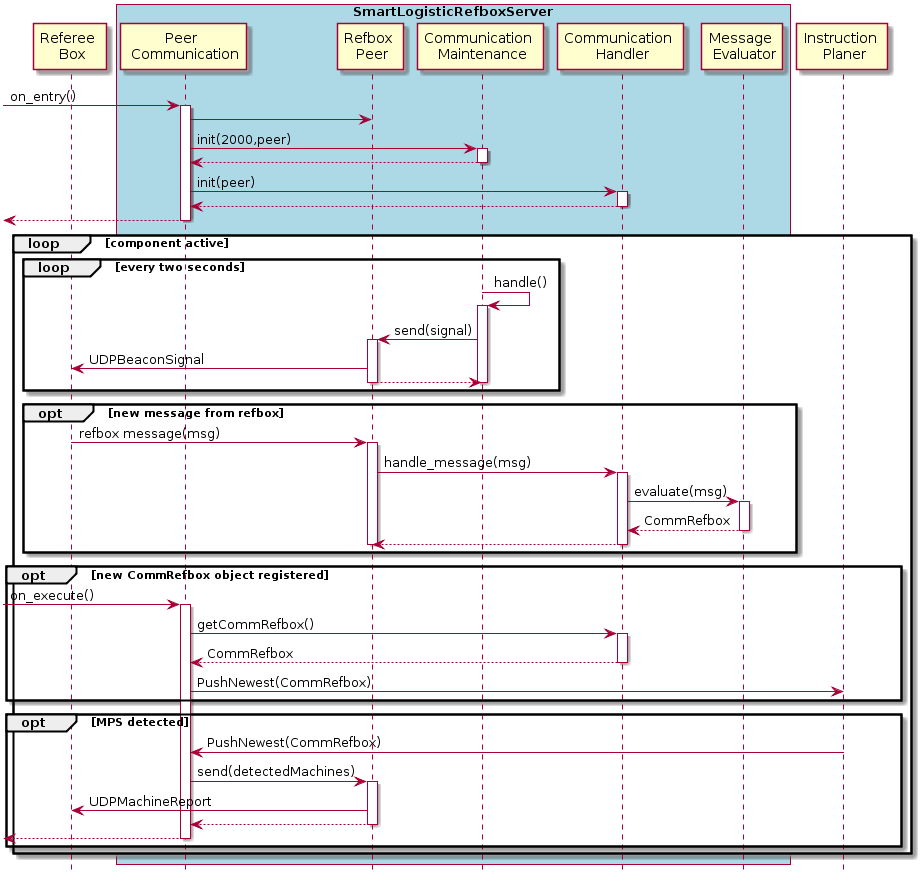
\includegraphics[width=\linewidth]{pic/sequence_diagram_RefboxServer.png}
\caption{Sequence diagram of Refbox server \cite{BOK}}
\label{fig:sequenceDiagramRefboxServer}
\end{figure}


\subsubsection{Difficulties}

On the Refbox server, the encryption was different during the competition than in the laboratory. At the Robocup competition, AES with Electronic Codebook Encryption (ECB) was used while Cipher Block Chaining (CBC) encryption was used by the Refbox installed in the laboratory. Therefore, one has to keep in mind to change the cipher method to the correct version at the competition. \\